\documentclass[a4paper,11pt]{article}
\usepackage[utf8]{inputenc}
\usepackage{geometry}
\geometry{left=4.0cm, right=4.0cm, top=4.0cm, bottom=3.5cm}
\usepackage[onehalfspacing]{setspace} 
\usepackage{graphicx}
\usepackage{tabularx}
\usepackage{hyperref}
\usepackage{float} 
\usepackage{ragged2e} %% Block justification
\usepackage{minted}
\usepackage[english]{babel}
\usepackage{xurl}


\usepackage{natbib}
\bibliographystyle{plainnat}





\title{Personalizing Climate Change: A Study on Instagram Polling Ads}

\begin{document}
\justifying
\pagenumbering{Roman}

\begin{titlepage}
    \centering
    {\Huge \textbf{Personalizing Climate Change:}\\[0.3cm] 
    \textbf{A Study on Instagram Polling Ads}}\\[1.5cm] % Title

    {\Large \textbf{Project Report}}\\[2cm] % Subtitle

    \textbf{Team Members:}\\[0.5cm]
    {\Large Najia Gul - 7062138}\\[0.3cm]
    {\Large Abaad Murtaza - 7061948}\\[2cm]

    \vfill

    {\large \today}
\end{titlepage}

\renewcommand{\contentsname}{Table of Contents}
\tableofcontents
\newpage

\pagenumbering{arabic}

%%%%%%%%%%%%%%%%%%%%%%%%%%% INTRODUCTION %%%%%%%%%%%%%%%%%%%%%%%%%%% 
\section{Abstract}
Climate change communication strategies often struggle to engage the public effectively, particularly in translating abstract global threats into personally relevant concerns. This study investigates whether localized, contextualized climate messaging—tailoring messages to specific regional landmarks—generates greater public concern compared to generic climate messaging using Instagram video polling ads. To test this, video ads featuring urban and rural landmarks in Germany were deployed, accompanied by polling questions measuring concern for climate change.
A/B testing using two-proportion z-tests found no statistically significant difference in concern levels between localized and generic messaging. However, Bayesian analysis estimated a 40.6\% probability that localized ads perform better, indicating high uncertainty due to the small sample size and unbalanced exposure between ad types. Additionally, gender differences emerged, with female respondents (74\%) expressing greater concern than males (53\%), suggesting that demographic factors may play a more significant role in engagement than localization alone.
Despite the inconclusive results, the study highlights the potential of Instagram video polling ads as a scalable, interactive tool for climate communication research. Future research with larger, more balanced datasets and controlled experimental conditions is necessary to fully assess whether localized climate messaging can effectively enhance public concern and engagement. These findings contribute to ongoing efforts in refining digital climate communication strategies to maximize impact across diverse audience segments.

%%%%%%%%%%%%%%%%%%%%%%%%%%%%%%%%%%%%%%%%%%%%%%%%%%%%%%%%%%%%%%%%%%%%

%%%%%%%%%%%%%%%%%%%%%%%%%%% INTRODUCTION %%%%%%%%%%%%%%%%%%%%%%%%%%% 
\section{Introduction}
Climate change has emerged as one of the most pressing and complex global challenges of the 21st century. Despite the overwhelming scientific consensus on the human impact on the Earth's climate, public concern and willingness to act remain inconsistent, varying across different regions, demographic groups, and media platforms. Scientific studies have demonstrated that effective climate communication can influence public understanding and action, yet many traditional approaches struggle with engagement, clarity, and lasting impact. This discrepancy—between the urgency of the crisis and the public’s often limited concern—highlights the need for more targeted and interactive climate communication strategies.

Social media, especially platforms like Instagram, has become a key tool for raising awareness and engaging audiences on social issues, including climate change. However, the effectiveness of interactive climate communication methods, such as polling ads, remains underexplored. Prior research suggests that localized and personalized climate messaging can enhance engagement, yet it remains unclear whether such an approach significantly increases public concern when delivered through social media platforms. Additionally, little research has examined whether demographic factors—such as age and gender—moderate the impact of localized climate messaging in an interactive format.

This project aims to explore the potential of Instagram video polling ads as a tool for climate change communication, with a particular focus on localized, personalized messaging. Specifically, this study will test whether tailoring climate change messages to specific regional impacts in Germany leads to greater public concern. Additionally, it will investigate how demographic factors, such as age and gender, influence audience responses to climate messaging. It is hypothesized that localized messages will lead to higher levels of concern than generic messages and that demographic characteristics will moderate this effect. Since this study was conducted in Germany, all ads were presented in German, inherently limiting participation to German-speaking users.

Building on prior research emphasizing the power of personalized, localized communication, this study incorporates interactive elements (i.e., polling questions) to add a real-time engagement component. Previous studies have shown that climate visuals with strong local relevance are more likely to capture attention and drive action. However, by integrating polling interactions, this research seeks to assess not just engagement levels, but also how messaging strategies translate into audience sentiment and concern.

This report is organized as follows: The \textbf{Abstract} provides a summary of the research objectives and key findings. The \textbf{Introduction} outlines the project’s background, aims, and significance. The \textbf{Literature Review} discusses existing research on climate change communication, the limitations of current approaches, and how this study fills key gaps. The \textbf{Methodology} section details the experimental design, data collection process, implementation, and analysis methods while the \textbf{Limitations and Challenges} section outlines constraints and potential biases in the study. Finally, the \textbf{Conclusion and Future Work} section summarizes the study’s contributions and proposes directions for future research.

%%%%%%%%%%%%%%%%%%%%%%%%%%%%%%%%%%%%%%%%%%%%%%%%%%%%%%%%%%%%%%%%%%% 

%%%%%%%%%%%%%%%%%%%%%% LITERATURE REVIEW %%%%%%%%%%%%%%%%%%%%%%%% 
\section{Literature Review}
Climate change communication has been the focus of extensive research, particularly in understanding how different messaging strategies influence public perceptions, engagement, and action. Existing literature explores various approaches, from communicating scientific consensus to analyzing the role of visual representation and social media engagement. However, key questions remain about the effectiveness of personalized and localized messaging in shaping public concern. This study builds on prior research by addressing these gaps through an experimental approach that tests contextualized climate messaging within Instagram polling ads.

One prominent area of research examines the impact of scientific consensus messaging on public attitudes toward climate change. \cite{Veckalov2024} conducted a 27-country study to determine whether emphasizing scientific agreement—either through a standard message ("97\% of scientists agree that human-caused climate change is real") or an extended crisis framing ("88\% of scientists call climate change a crisis")—could reduce misperceptions and increase support for climate action. The study found that while such messaging effectively increased perceptions of scientific consensus, its influence on deeper concern and policy support was limited. Moreover, message effectiveness varied significantly across political and cultural contexts, suggesting that a one-size-fits-all communication strategy may not be sufficient in driving meaningful public engagement. Although this study provides valuable insights into the role of expert consensus, it does not address whether making climate change personally relevant—by linking it to familiar places or cultural heritage—could be a more effective approach. This is where our research extends the conversation: rather than testing scientific authority-based framing, we examine whether localized and personally relevant messages enhance public concern, using behavioral engagement metrics from Instagram rather than survey-based perception changes.

Another significant strand of climate communication research focuses on the role of visual representation and engagement on social media. \cite{Leon2022} analyzed 380 climate-related images from Twitter, seeking to understand which types of visuals drive the most interaction. They found that traditional climate imagery, such as melting ice caps, often fails to elicit engagement. Instead, images featuring real people, compelling narratives, and local connections were significantly more effective at drawing user attention and fostering interaction. This aligns with broader theories in media studies, such as the availability heuristic, which suggests that people engage more with content they find personally meaningful. While this research highlights the importance of personalization in visual content, it primarily focuses on static images on Twitter. Our study builds on this by testing whether personalized messaging in text format—such as climate-related polling questions—can have a similar effect in increasing engagement and concern on Instagram. Additionally, while \cite{Leon2022} measured passive engagement (likes, shares, and comments), our study examines active engagement through polling responses, offering a stronger behavioral indicator of concern.

The growing role of social media in shaping climate discourse has also been explored in broader theoretical frameworks. \cite{Schaefer2024} provides a comprehensive review of climate change communication in digital spaces, highlighting both opportunities and challenges. On one hand, social media democratizes climate communication, allowing grassroots movements like Fridays for Future to bypass traditional media gatekeepers. On the other hand, algorithmic biases, echo chambers, and misinformation pose significant obstacles to effective climate messaging. Short-form content platforms such as TikTok have increased public exposure to climate-related narratives, but the study raises concerns about oversimplification, virality-driven distortion, and the influence of influencers with limited scientific expertise. While \cite{Schaefer2024}’s review provides a macro-level understanding of these digital trends, it lacks empirical testing of specific messaging strategies that could counteract disengagement. Our study contributes by empirically examining how localized climate messaging influences concern in a real-world social media setting, offering data-driven insights into how interactive content might overcome algorithmic biases and disengagement trends.

The challenge of effectively communicating climate change is further complicated by the pervasive nature of misinformation. \cite{Jiang2024} demonstrated that the repetition of climate denial claims can enhance their perceived credibility, even among individuals who support climate science. This "illusory truth effect" suggests that merely countering misinformation with factual statements may be insufficient, as repetition alone can lend undue credibility to false claims. This finding underscores the importance of strategic communication approaches that not only disseminate accurate information but also do so repetitively to reinforce its credibility. In this context, our study seeks to explore whether localized, contextualized messaging can serve as an effective strategy to enhance public concern and engagement with climate change, thereby countering the effects of misinformation.

While these studies provide valuable contributions to climate change communication, they leave critical gaps. Most research focuses on broad messaging strategies or content analysis, but few studies empirically test how audience interaction with different types of messaging unfolds in real-time on social media platforms. Furthermore, while there is recognition that personalized content fosters engagement, little is known about whether contextualized climate messaging—framing climate change in terms of local landmarks or cultural identity—can increase concern more than generic messaging. Our study bridges this gap by leveraging Instagram polling ads as an experimental setting, providing a novel test of message framing effectiveness within an interactive, high-engagement social media format.

Thus, this research extends prior work by shifting the focus from broad consensus messaging and static visual engagement to a localized, interactive approach that measures real-time shifts in public concern.

%%%%%%%%%%%%%%%%%%%%%%%%%%%%%%%%%%%%%%%%%%%%%%%%%%%%%%%%%%%%%%%%%%%%

\section{Methodology}
\subsection{Data Collection}
The data collection process was carefully designed to assess the impact of localized vs. generic climate change messaging using Instagram video polling ads. This process involved the creation, deployment, and monitoring of ad sets to capture audience responses across different demographic groups. The approach ensured that the data collected was both reliable and structured, allowing for meaningful comparisons between localized and generic messaging strategies.

\subsubsection{Video Ad Design and Development}
To test the effect of localized climate messaging, video ads were created for five German states, each featuring one urban and one rural location. Additionally, a generic climate change ad was produced, which did not reference any specific location. The selection of these locations ensured regional diversity and provided a comprehensive basis for assessing the differences between urban and rural engagement with climate messaging.

The selected locations and their associated landmarks included:

\begin{table}[H]
\centering
\small % Reduce font size
\renewcommand{\arraystretch}{1.2} % Increase row height for better readability
\setlength{\tabcolsep}{3pt} % Reduce column padding to prevent shifting

\begin{tabular}{|p{3.2cm}|p{4.5cm}|p{4.5cm}|} 
    \hline
    \textbf{State} & \textbf{Urban City (Landmark)} & \textbf{Rural Area (Landmark)} \\ \hline
    North 
    
    Rhine-Westphalia & Cologne 
    
    (Cologne Cathedral) & Höxter District 
    
    (Schloss Corvey) \\ \hline
    Bavaria & Munich 
    
    (English Garden) & Oberpfalz 
    
    (Wallaha Memorial) \\ \hline
    Baden-Württemberg & Stuttgart 
    
    (Stuttgart's Schlossplatz) & Schwarzwald 
    
    (Black Forest) \\ \hline
    Hesse & Frankfurt am Main 
    
    (Stadtwald) & Vogelsbergkreis 
    
    (Hinterturm) \\ \hline
    Saarland & Saarbrücken 
    
    (Saar River) & Blieskastel (Schlosskirche St. Anna und St. Philipp) \\ \hline
\end{tabular}

\caption{Selected locations for localized climate messaging}
\label{tab:selected_locations}
\end{table}





Each video was carefully designed to follow a consistent format, ensuring that the messaging remained cohesive and engaging across different locations. \\

\noindent \textbf{Initial Visual Presentation}
\begin{itemize}
    \item The video opened with a visual representation of the selected landmark in its normal state, providing instant recognition for viewers.
\end{itemize}

\noindent \textbf{Filter-Based Visual Degradation}
\begin{itemize}
    \item To illustrate the impact of climate change, filters were applied to modify the landmark’s appearance, making it look worn, discolored, or deteriorated.
    \item This technique was used instead of portraying disasters like flooding or extreme weather to create a subtle yet powerful visual cue.
\end{itemize}

\noindent \textbf{Dramatic Background Music}
\begin{itemize}
    \item Each video was accompanied by relevant dramatic background music to enhance the emotional impact of the message.
    \item The music was selected to complement the visuals, drawing attention to the urgency of climate change and reinforcing the seriousness of the message.
\end{itemize}

\noindent \textbf{Call to Action (CTA) Overlay}

As the altered image appeared, a Call to Action (CTA) text overlay was displayed, reinforcing the potential risk posed by climate change. The CTA text was customized based on the ad type:\\

\textbf{I. Localized (Contextualized) CTA Example:}
\begin{quote}
    \textbf{Klimawandel bedroht den Kölner Dom. Schützen wir unser Erbe.} \\
    \textit{Translation:} \\
    “Climate change threatens Cologne Cathedral. Let’s protect our heritage.”
\end{quote}

\textbf{II. Generic CTA Example:}
\begin{quote}
    \textbf{Klimawandel bedroht unsere Zukunft. Handeln wir jetzt.} \\
    \textit{Translation:} \\
    “Climate change threatens our future. Let’s act now.”
\end{quote}

\noindent \textbf{Polling Question Integration}

At the end of both contextualized and generic ads, users were presented with the same Yes/No polling question:

\begin{quote}
    \textbf{Glauben Sie, dass der Klimawandel eine ernsthafte Bedrohung ist?} \\
    \textit{Translation:} \\
    “Do you think climate change is a serious threat?”
\end{quote}

This uniform polling question allowed for direct comparisons between different ad variations, ensuring that any observed differences in responses were due to the messaging approach rather than differences in the question itself.

This structured approach to video design ensured that the messaging was consistent, engaging, and scientifically grounded, while also providing a measurable way to assess audience sentiment through polling responses.

\subsubsection{Ad Deployment Phase}
The ads were launched exclusively on Instagram, utilizing targeted advertising features to ensure the right audience was reached. The deployment was controlled and systematic, focusing on gathering accurate engagement metrics across different demographic segments.

\subsubsection{Polling Interaction and Data Collection}
Polling responses were the primary data collection method, allowing the study to capture quantitative insights into public concern about climate change. Three key engagement metrics were monitored:\\

\noindent \textbf{I. Ad Reach}
\begin{itemize}
    \item The total number of Instagram users who viewed the ad, providing an estimate of overall exposure.
\end{itemize}

\noindent \textbf{II. Poll Participation Rate}
\begin{itemize}
    \item The number of users who actively responded to the Yes/No polling question, indicating direct engagement with the climate messaging.
\end{itemize}

\noindent \textbf{III. Demographic-Based Engagement Trends}
\begin{itemize}
    \item Variations in responses were recorded based on age and gender categories, helping to identify which groups were more receptive to localized messaging.
\end{itemize}

\subsection{Setup}
Although video ads were created for all ten locations, the experimental setup focused on two selected cities—Cologne and Blieskastel, representing urban and rural environments, respectively. This was due to budget constraints and copyright limitations. The selection was based on the availability of copyright-free visual material, ensuring that the content met advertising policies. This setup limited the analysis of how geographic factors influenced engagement and climate concern.

\subsubsection{Selection of Cities and Controlled Deployment}
Cologne was chosen as the urban location, given its high population density and historical significance. Blieskastel, a rural area with lower population density, was selected to represent engagement trends in less urbanized settings. The deployment in these two cities was designed to provide insights into how different audiences perceive climate messaging when it is tailored to familiar locations.

\subsubsection{Demographic Segmentation and Targeting}
To ensure diversity in audience engagement, the study followed a structured segmentation approach based on age and gender, as represented in the flowchart.

\begin{figure}[H]
    \centering
    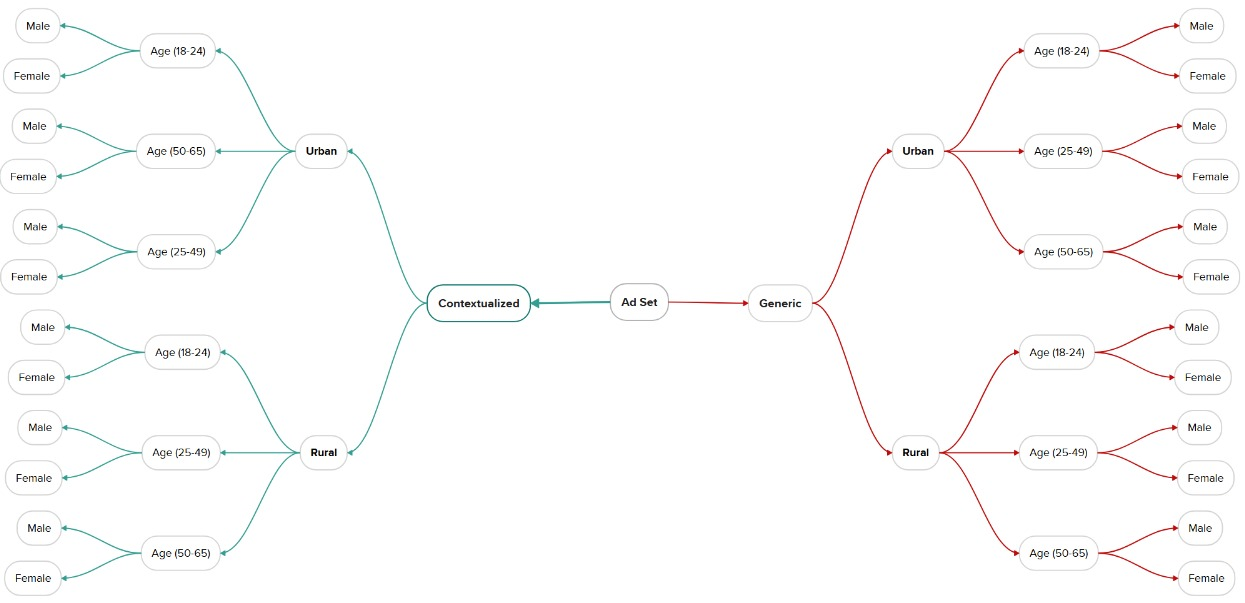
\includegraphics[width=1\textwidth]{demographic_segmentation_flowchart.png} 
    \caption{Demographic segmentation and targeting}
    \label{fig:demographic_segmentation}
\end{figure}

\noindent The ads were divided into two primary categories:

\paragraph{I. Contextualized (Localized) Ads}
\begin{itemize}
    \item These ads were further subdivided into urban (Cologne) and rural (Blieskastel) settings.
    \item Each city’s ad was targeted to three distinct age groups:
    \begin{itemize}
        \item 18–24 years
        \item 25–49 years
        \item 50–65 years
    \end{itemize}
    \item Each age group was further segmented by gender, ensuring equal distribution of ads to male and female audiences.
\end{itemize}

\paragraph{II. Generic Ads}
\begin{itemize}
    \item The generic climate ad was deployed in both urban and rural locations, maintaining the same age and gender segmentation structure as the contextualized ads.
\end{itemize}

By structuring the ad deployment in this way, the study ensured that data collection was systematic, allowing for precise comparisons between localized and generic climate messaging across different demographic groups.

\subsection{Data Analysis and Discussion}
After running the Instagram polling ads, the study collected audience engagement data across different demographic groups. The dataset comprised responses from two cities—Cologne (urban) and Blieskastel (rural)—with polling results categorized by age group, gender, and ad type (Contextualized vs. Generic).

The key engagement metrics recorded were:
\begin{itemize}
    \item \textbf{Ad Reach}: Number of users who viewed the ad.
    \item \textbf{Yes Responses}: Number of users who answered "Yes" to the question: “Do you think climate change is a serious threat?”
    \item \textbf{No Responses}: Number of users who answered "No" to the same question.
\end{itemize}

The collected dataset was relatively small, particularly for Generic ads, which received less reach and fewer total responses compared to Contextualized ads. This imbalance in exposure presented challenges in making direct comparisons. Despite this, the study proceeded with A/B testing and Bayesian inference to analyze trends and extract meaningful insights.


\subsubsection{A/B Testing (Two-Proportion Z-Test)}
To compare engagement levels between Contextualized and Generic ads, we performed two-proportion z-tests. These tests assessed whether the proportion of "Yes" responses was significantly different between the two ad types.


\paragraph{Hypotheses for A/B Testing}
\begin{itemize}
    \item \textbf{Null Hypothesis (\(H_0\))}: There is no difference in the proportion of "Yes" responses between Contextualized and Generic ads. (\( p_A = p_B \))
    \item \textbf{Alternative Hypothesis (\(H_1\))}: The proportion of "Yes" responses is different for the two ad types. (\( p_A \neq p_B \))
\end{itemize}


\paragraph{Results from A/B Testing} 


\subsubsection*{I. Subgroup-Specific Tests}
A/B testing was conducted for subgroups where both Contextualized and Generic ads existed. \\
One example: \textbf{Blieskastel, Female, 25-49}

\begin{table}[H]
\centering
\begin{tabular}{|l|c|c|}
    \hline
    \textbf{Group} & \textbf{Yes} & \textbf{No} \\ \hline
    Contextualized Ads  & 5 & 0 \\ \hline
    Generic Ads & 4 & 1 \\ \hline
\end{tabular}
\caption{Example A/B Test Subgroup Data}
\end{table}

\noindent \textbf{Statistical Results:}
\begin{itemize}
    \item \textbf{Z-statistic}: 1.0541
    \item \textbf{p-value}: 0.2918
\end{itemize}
Since the p-value exceeded the 0.05 threshold, we failed to reject the null hypothesis, meaning no statistically significant difference was observed.

\subsubsection*{II. Aggregated A/B Test Across All Data} 
\begin{table}[H]
\centering
\begin{tabular}{|l|c|c|}
    \hline
    \textbf{Group} & \textbf{Yes} & \textbf{No} \\ \hline
    Contextualized Ads & 41 & 31 \\ \hline
    Generic Ads & 8 & 5 \\ \hline
\end{tabular}
\caption{Aggregated A/B Test Results}
\end{table}

\noindent \textbf{Statistical Results:}
\begin{itemize}
    \item \textbf{Z-statistic}: -0.3085
    \item \textbf{p-value}: 0.7577
\end{itemize}
The aggregated test across all responses also failed to show statistical significance. This result suggests that, given the small sample size, the observed differences between Contextualized and Generic ads may have occurred by chance rather than due to a real effect.

\subsubsection{Bayesian A/B Testing}
Given the low sample size, traditional significance testing lacked the statistical power to detect meaningful differences. To overcome this limitation, we conducted Bayesian inference to estimate the probability that Contextualized ads were better than Generic ads in terms of generating "Yes" responses.

\paragraph{Bayesian Inference Model}
\begin{itemize}
    \item We modeled the Yes/No responses as probabilities using Beta distributions, a common prior for Bayesian A/B testing.
    \item We assumed uninformative priors (\(\alpha = 1, \beta = 1\)) to avoid biasing results toward either ad type.
    \item Using 10,000 posterior samples, we calculated the probability that Contextualized ads had a higher conversion rate than Generic ads.
\end{itemize}

\begin{figure}[H]
    \centering
    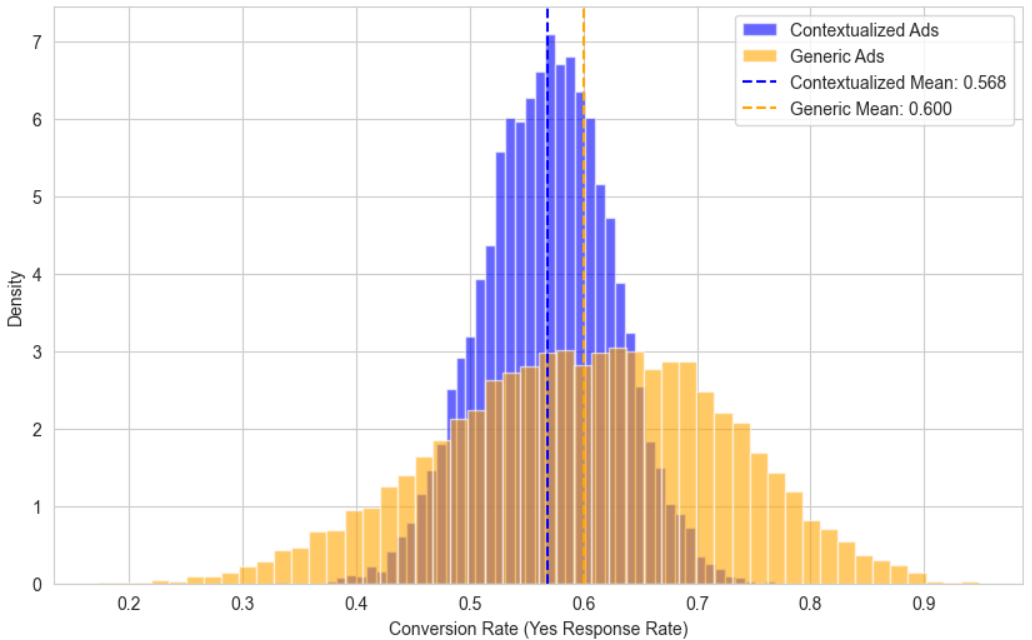
\includegraphics[width=1\textwidth]
    {posterior_distribution.png} 
    \caption{Posterior Distribution for Centextualized vs Generic Ads}
    \label{fig:Posterior Distribution for Centextualized vs Generic Ads}
\end{figure}

\paragraph{Results from Bayesian Inference}
\begin{itemize}
    \item \textbf{Estimated Probability}: Contextualized Ads outperform Generic Ads in 40.6\% of simulations.
    \item Since this is below the 50\% threshold, Generic ads had a slightly higher success rate.
    \item The probability distributions of Contextualized and Generic ads largely overlapped, indicating high uncertainty.
\end{itemize}
Bayesian inference reinforces the finding that more data is needed to make a definitive conclusion about ad effectiveness.


\subsubsection{Gender-Based Analysis}
Another key insight emerged when analyzing responses by gender:
\begin{itemize}
    \item \textbf{Female respondents} had a higher concern rate (\textbf{74\%}) compared to males (\textbf{53\%}).
\end{itemize}
This suggests that women may be more responsive to climate messaging, though further research is needed to determine whether this effect is consistent across larger samples.

\begin{figure}[H]
    \centering
    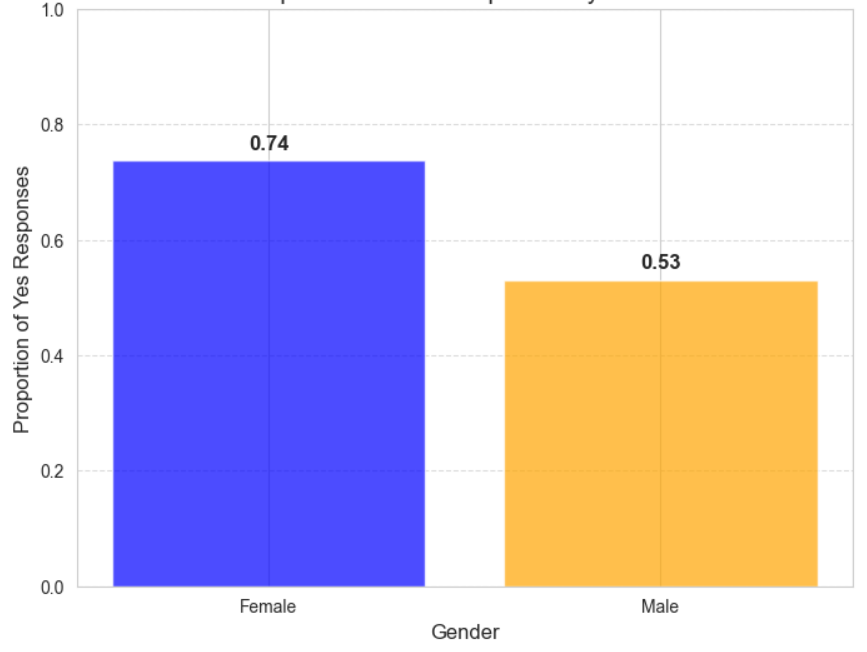
\includegraphics[width=1\textwidth]
    {yes_responses_by_gender.png} 
    \caption{Proportion of 'Yes' Responses by Gender}
    \label{fig:Posterior Distribution for Centextualized vs Generic Ads}
\end{figure}

\subsubsection{Key Findings}
\begin{itemize}
    \item Traditional A/B testing found no significant differences between Contextualized and Generic ads.
    \item Bayesian analysis estimated a 40.6\% probability that Contextualized ads perform better, indicating high uncertainty due to small sample size.
    \item \textbf{Proportion of 'Yes' Responses by Gender:}
    \begin{itemize}
        \item \textbf{Females:} 74\% concern rate.
        \item \textbf{Males:} 53\% concern rate.
    \end{itemize}
    \item These results suggest potential demographic differences in climate messaging engagement.
\end{itemize}


\section{Challenges and Limitations}
The experimental setup aimed to create a controlled A/B testing environment to assess the impact of localized vs. generic climate messaging. However, several challenges and inconsistencies affected the overall validity of the experiment, requiring careful consideration when interpreting the results. These issues ranged from technical limitations in ad creation and deployment to methodological inconsistencies in the A/B testing setup.

\subsection{Challenges in Ad Creation and Deployment}
A key challenge during ad development was the availability of high-quality, open-source images for rural locations. While images for urban landmarks were more widely accessible, sourcing license-free visuals for rural landmarks proved difficult. This limitation affected the visual consistency of the ads, as some rural locations lacked the same level of high-quality imagery as their urban counterparts. Ensuring equal visual appeal and clarity across all ad variations was necessary to maintain comparability, but the differences in available resources may have influenced engagement levels.

Another major constraint was Facebook’s ad approval process, as some ads were flagged under the platform’s "social issue policies". Climate change falls under Facebook’s regulated ad categories, requiring additional verification and compliance. Some ads were initially rejected, delaying the deployment process and reducing the overall dataset. These restrictions limited ad reach and required modifications in ad content to meet Facebook’s policies, impacting data consistency.

Additionally, Instagram’s ad delivery algorithm resulted in uneven exposure across demographic groups. Some age and gender categories received significantly higher engagement than others, suggesting that the platform's algorithm may have optimized ad delivery toward users more likely to interact with climate content. This uneven reach required refined targeting strategies in future studies to ensure a balanced sample across all demographic segments.

\subsection{Budget and Sample Size Constraints}
The study was conducted with a €120 budget, which limited the scope of ad placements and audience reach. While the budget allowed for preliminary insights, it restricted the total sample size, affecting the statistical power of the results. A larger budget would have enabled ads to be deployed in all ten selected cities, increasing the representativeness of the data. Additionally, a higher budget could have ensured more impressions per demographic group, reducing engagement biases caused by uneven ad reach.

\subsection{Mistakes in A/B Testing Setup}
A critical limitation in the experimental setup was the variation in background music across different ad videos. In an ideal A/B testing framework, all variables except for the independent variable (localized vs. generic messaging) should remain constant. However, due to an oversight, each ad featured different background music, which was not intended as a variable in the study.

Since music can evoke emotional responses, its variation across ad versions may have influenced audience perception and engagement levels, introducing uncontrolled variability in the results. Future studies should ensure that all non-experimental factors, including background audio, remain identical across ad versions to maintain experimental validity.

\subsection{Language Restriction and Audience Representation}
Another significant limitation was the exclusive use of the German language in all ads. Since the ads were specifically designed for a German audience, they were only accessible to German-speaking users, which naturally restricted the number of potential respondents. While this approach ensured linguistic consistency, it also excluded non-German speakers, limiting the generalizability of the findings beyond German-speaking regions.

Future research could consider multi-language ad campaigns or include subtitle options to assess whether language barriers influence engagement with climate messaging. This would provide insights into cross-cultural differences in climate concern and public perception when exposed to localized vs. generic messaging.

\section{Conclusion}
Effective climate change communication remains a pressing challenge, particularly in fostering public engagement and concern. This study explored the potential of localized, contextualized climate messaging by testing whether region-specific messaging tied to local landmarks increases concern about climate change compared to generic messaging. Utilizing Instagram video polling ads, we measured real-time audience engagement and analyzed responses through A/B testing (two-proportion z-tests) and Bayesian inference.

The findings were inconclusive, primarily due to small sample size and unbalanced ad exposure. Traditional hypothesis testing failed to detect statistically significant differences between localized and generic messages, and Bayesian analysis estimated only a 40.6\% probability that localized ads perform better, suggesting high uncertainty. However, a notable gender disparity emerged, with female respondents (74\%) showing greater concern than males (53\%), implying that demographic factors may influence engagement more than message localization alone.

Despite these limitations, this study highlights the potential of Instagram video polling ads as an interactive, scalable tool for climate change communication and research. The platform allows for real-time audience engagement tracking, making it a valuable resource for testing different framing strategies and demographic variations in climate messaging.

\bibliography{references}


\end{document}
